%%%%%%%%%%%%%%%%%%
\section{多视图聚类简介}


\begin{frame}
    \frametitle{多视图聚类}
    \begin{itemize}
        \item 多视图聚类:利用多个视图上的信息来弥补单一视图上可能的信息不足的问题
            \begin{itemize}
            \item 例如对于一个网页而言,它具有多种数据形式:文本,图片,超链接等等。每种数据形式都可以被用来对网页进行分类,即每种数据形式都可以被看做该网页的一个视图。


            \end{itemize}
        \item 多视图的优越性:信息的互补性,使得其潜在的表示能力增强
         \begin{itemize}
         \item 给多个视图的情况下,我们如何得到最优的聚类结果
         \end{itemize}
        \end{itemize}
\end{frame}

\begin{frame}
    \frametitle{早期方法}
    \begin{itemize}
        \item 将所有视图上的特征组合起来做聚类方法,比如$k$-means和谱聚类;
        \item 借鉴集成学习的思路,将多个聚类结果集成到最终聚类结果
    \end{itemize}
\end{frame}


\begin{frame}
    \frametitle{后期融合 late fusion}
    \begin{itemize}
        \item 中期融合是利用多个视图上得到的不同相似度信息统一到相似度矩阵上去,;
        \item 现有的多视图聚类算法:
              \begin{itemize}
                 \item 基于图的(graph-based):通过融合各个视图上的图得到最优的图表示
                 \item 基于子空间的(subspace learning):将多个视图上的表示通过优化目标得到一个潜在的共同空间表示(low-rank,sparse等等)
                 \item 基于多核的:将多个核矩阵融合成一个统一的核矩阵
                 \item 基于非负矩阵分解(NMF)的:将每个视图的低阶表示对齐到一个表示上
              \end{itemize}

    \end{itemize}
\end{frame}

\begin{frame}
    \frametitle{后期融合 late fusion}
    \begin{figure}[!ht]
\begin{center}
{
\centering
\subfloat[]{{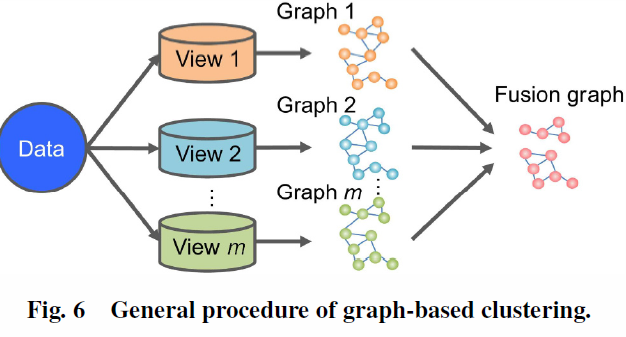
\includegraphics[width=1\textwidth]{figures/graph.png}} \label{figure_clustering}}
\caption{基于图的多视图聚类.}
\label{figure_evaluation_objective one}
}
\end{center}
\end{figure}
\end{frame}

\begin{frame}
    \frametitle{后期融合 late fusion}
    \begin{figure}[!ht]
\begin{center}
{
\centering
\subfloat[]{{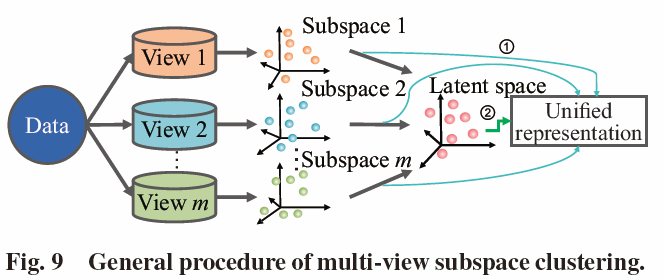
\includegraphics[width=1\textwidth]{figures/subspace.png}} \label{figure_convergence}}
\caption{基于子空间的多视图聚类}
\label{figure_evaluation_objective one}
}
\end{center}
\end{figure}
\end{frame}

\begin{frame}
    \frametitle{后期融合 late fusion}
    \begin{figure}[!ht]
\begin{center}
{
\centering
\subfloat[]{{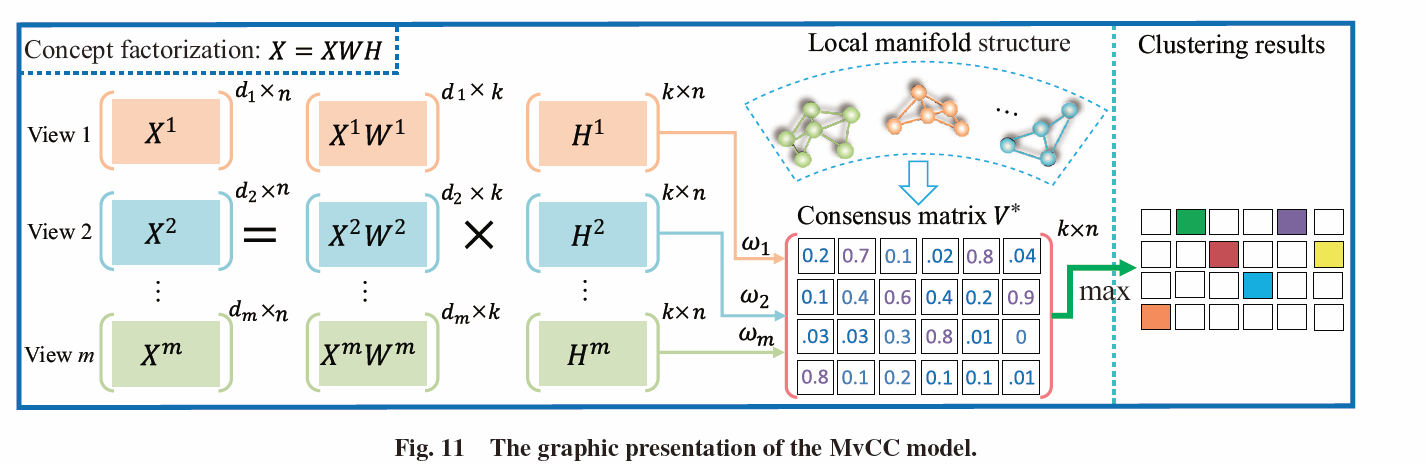
\includegraphics[width=1\textwidth]{figures/nmf.png}} \label{figure_parameter}}
\caption{基于非负矩阵分解的多视图聚类}
\label{figure_evaluation_objective one}
}
\end{center}
\end{figure}
\end{frame}

\begin{frame}
    \frametitle{后期融合 late fusion}
    \begin{figure}[!ht]
\begin{center}
{
\centering
\subfloat[]{{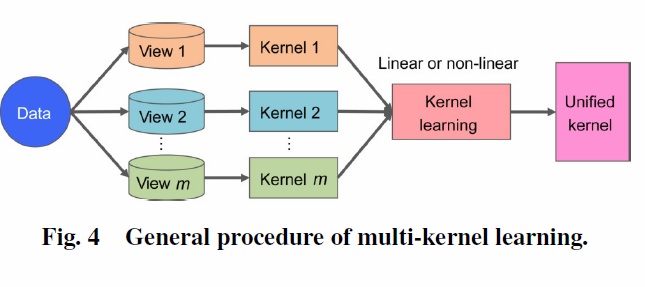
\includegraphics[width=1\textwidth]{figures/multi-kernel.png}} \label{figure_parameter}}
\caption{基于多核的多视图聚类}
}
\end{center}
\end{figure}
\end{frame}

\begin{frame}
    \frametitle{后期融合}
    \begin{itemize}
        \item 缺陷:中期融合的方法时间和空间复杂度相对都比较高,因为往往需要对相似度矩阵做SVD分解,这意味着空间复杂度为$\mathcal{O}(m n^2)$,时间复杂度为$\mathcal{O}( n^3)$;
        \item 动机:类似于ensemble learning的思想,将若干视图上取得任务结果做聚类语义上的对齐;
        \item 这里的聚类结果对应 $\{\mathbf{V}_{i}\}_{i=1}^{m}$所产生的$m$个聚类指示矩阵$\{\mathbf{H}_{i}\}_{i=1}^{m}$
        \item novelty:无监督的无标签性      
    \end{itemize}      
\end{frame}


\begin{frame}
    \frametitle{后期融合}
    \begin{itemize}
        \item 不同聚类结果之间的距离不能简单靠相减计算。
        \item 假设我们现在有5个样本和三个簇。我们从两个视图上得到了各自视图上的聚类结果如下,
\[
\mathbf{H_{1}} = \left|\begin{array}{cccc}
    1 &    0    & 0 \\
    1 &    0   & 0\\
    0 &    1   & 0 \\
    0 &    1   & 0 \\
    0 &    0   & 1
\end{array}\right|,
 \mathbf{H_{2}} = \left|\begin{array}{cccc}
    0 &    0    & 1 \\
    0 &    0   &  1\\
    1 &    0   &  0\\
    1 &    0   &  0\\
    0 &    1   &  0
\end{array}\right|
\]   
       \item 尽管数学表达形式不同,但是聚类结果一致
    \end{itemize}      
\end{frame}

\begin{frame}
    \frametitle{后期融合}
    \begin{itemize}
        \item 所以我们不能单纯地用数学意义上的范数来评估两个矩阵的相似性。对于聚类指示矩阵而言,只要能够通过列变换矩阵得到的新的聚类结果,就可以被看做与原结果等价
        \item $\mathbf{H_1} = \mathbf{H_2}\mathbf{W_2}$ 
\[
\mathbf{W_{2}} = \left|\begin{array}{cccc}
    0 &    1    & 0 \\
    0 &    0   & 1\\
    1 &    0   & 0
\end{array}\right|
\]      
    \end{itemize}      
\end{frame}

\begin{frame}
    \frametitle{后期融合}
    \begin{itemize}
        \item 优化目标
 \begin{equation}
\label{MKKM LF3}
\begin{split}
\min\limits_{\mathbf{H},\left\{\mathbf{W_p}\right\}_{p=1}^m}{\left\lVert\mathbf{H} - \frac 1m \sum_{p=1}^m \mathbf{H}_p \mathbf{W}_p\right\rVert}_{\mathbf{F}}^2,\\ ~~
s.t. ~~  \mathbf{H^{\top}}\mathbf{H} = \mathbf{I}_k, \mathbf{W^{\top}}\mathbf{W} = \mathbf{I}_k.
\end{split}
\end{equation}  

\begin{equation}
\label{MKKM LF4}
\begin{split}
\min\limits_{\mathbf{H},\left\{\mathbf{W}_p\right\}_{p=1}^m,\gamma}{\left\lVert\mathbf{H} - \sum_{p=1}^m \gamma_p \mathbf{H}_p \mathbf{W}_p\right\rVert}_{\mathbf{F}}^2,\\ ~~
s.t. ~~  \mathbf{H^{\top}}\mathbf{H} = \mathbf{I}_k, \mathbf{W^{\top}}\mathbf{W} = \mathbf{I}_k,
 \gamma^{\top}1=1,\gamma \geq 0.
\end{split}
\end{equation}   
    \end{itemize}      
\end{frame}

\begin{frame}
    \frametitle{后期融合算法}
    \begin{itemize}
        \item 后期融合通过每个视图下得到的聚类的结果,通过不同的聚类结果融合成最终的最优结果
        \item 我们是通过列变换对齐的,只要满足聚类的性质,这种对齐就可以被应用到其他领域的聚类算法上
    \end{itemize}     
      
\end{frame}
